\markdownRendererHeadingFour{Arquitectura}\markdownRendererInterblockSeparator
{}\begin{figure}[h!] \centering 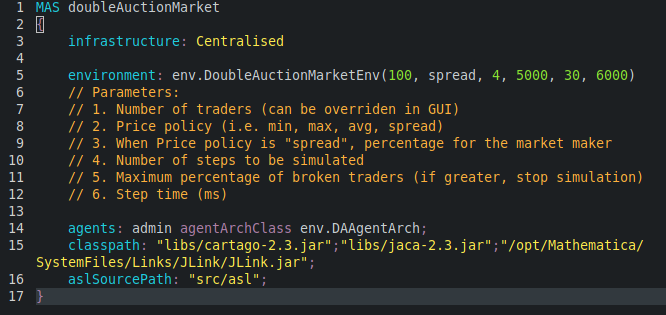
\includegraphics[scale=0.3]{img/code.png} \end{figure}\markdownRendererInterblockSeparator
{}\markdownRendererUlBegin
\markdownRendererUlItem La simulación se realiza en un ambiente llamado \markdownRendererEmphasis{DoubleAuctionMarketEnv}.\markdownRendererUlItemEnd 
\markdownRendererUlItem Este ambiente comienza levantando CArtAgO, y genera un artefacto GUI que recibe parámetros del usuario (ambiente externo).\markdownRendererUlItemEnd 
\markdownRendererUlItem En cuanto el artefacto envía la señal de comenzar, el administrador crea a los traders, envía parámetros, y finaliza terminando su existencia y cerrando los servicios CArtAgO.\markdownRendererUlItemEnd 
\markdownRendererUlItem Comienza la simulación en el ambiente usando \markdownRendererEmphasis{acciones internas}.\markdownRendererUlItemEnd 
\markdownRendererUlEnd \markdownRendererInterblockSeparator
{}\markdownRendererHorizontalRule{}\markdownRendererInterblockSeparator
{}\markdownRendererHeadingFour{Simulación de precios}\markdownRendererInterblockSeparator
{}Al evaluar los resultados añadiendo mayor proporción de agentes que siguen la estrategia Moving Average (MA) se observa que el comportamiento de la serie de tiempo de precios adquiere periodicidad hasta llegar a un punto crítico entre 75\% y 80\% de agentes MA en donde la simulación converge a un precio estacionario.\markdownRendererInterblockSeparator
{}\begin{figure}[h!] \centering 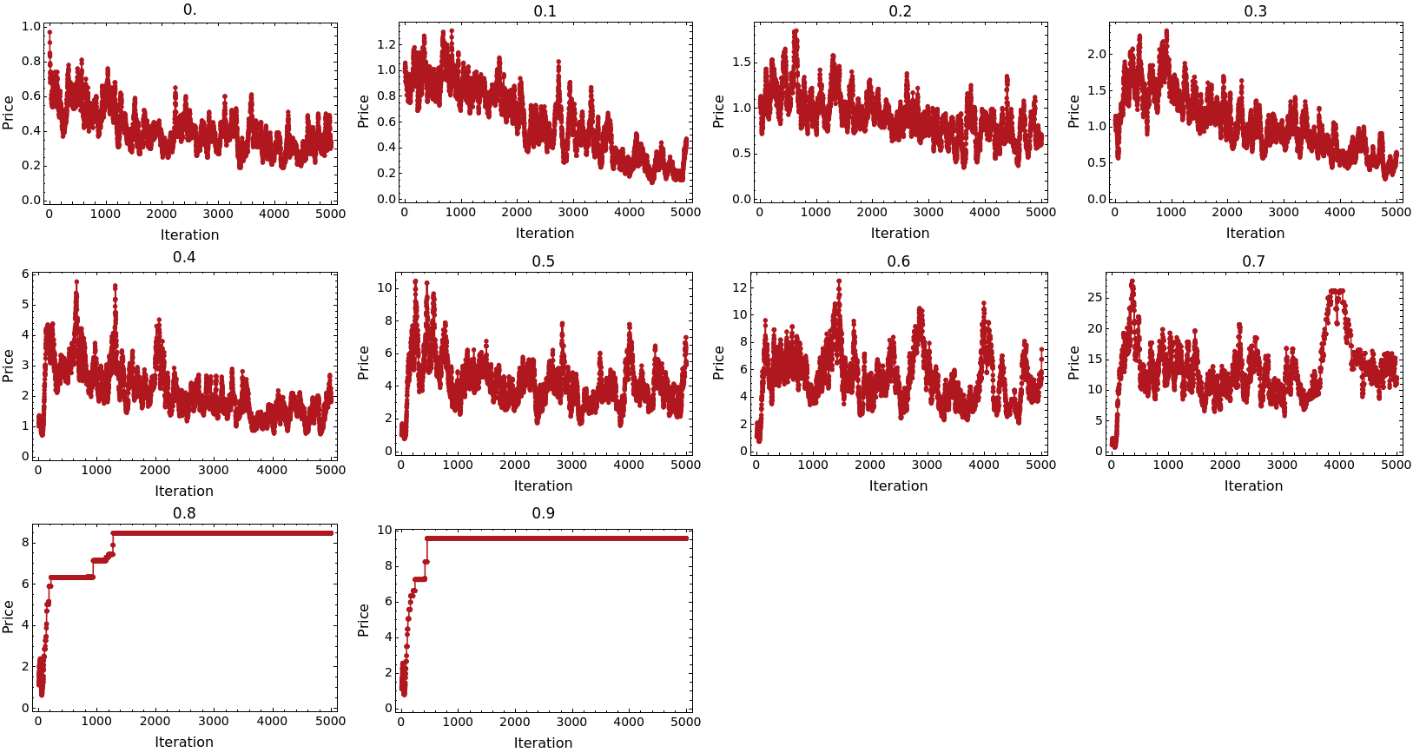
\includegraphics[scale=0.25]{img/price_series.png} \end{figure}\markdownRendererInterblockSeparator
{}\markdownRendererHorizontalRule{}\relax